\subsection{Tracking Overview}

Charged particle tracking is the key element of the CLAS12 event reconstruction. It is separated into the
reconstruction of tracks in the central tracker system (comprised of the Silicon Vertex Tracker - SVT
\cite{svt-nim} and the Barrel Micromegas Tracker - BMT~\cite{mm-nim}; together the SVT and BMT comprise
the Central Vertex Tracker - CVT)  and the forward tracking system (comprised of the Forward Micromegas
Tracker - FMT~\cite{mm-nim} and the Drift Chambers - DCs~\cite{dc-nim}). The Forward Detector covers the
polar angle range from $5^\circ$ to $40^\circ$, while the Central Detector covers the polar angle range from
roughly $40^\circ$ to $135^\circ$. In the forward region a torus magnet bends charged particles inward toward
the beamline or outward away from the beamline depending on their charge. At full nominal current the $\int B dl$
varies from roughly 2~Tm at 5$^\circ$ to 0.5~Tm at 40$^\circ$. In the central region a 5~T solenoidal magnetic
field bends charged tracks into helices. A view of the field intensities in the $(z,x)$ plane and overlap region for
the torus and solenoid fields is shown in Fig.~\ref{fig:dcTracks}.

For both systems, track reconstruction comprises algorithms for pattern recognition and track fitting. Hit objects,
corresponding to the passage of a particle through a particular detector component, require the transformation of
an electronic signal into a location of the track's position in the detector subsystem geometry. A hit is thus a
geometric object, for example, a line segment. These objects then form the input to the pattern recognition
algorithms. This first step involves the identification of clusters of hits and the determination of the spatial
coordinates and corresponding uncertainties for the hits and clusters of hits. At the pattern recognition stage, hits
that are consistent with belonging to a trajectory (i.e. track) are identified. This set of hits is then fit to the
expected trajectory with their uncertainties, incorporating the knowledge of the detector material and the
detailed magnetic field map.

\subsection{Forward Tracking}

\subsubsection{Hit Reconstruction}
\label{sec:hitrecon}

The Drift Chamber (DC) wire hit information is given by the wire geometrical location and the drift time to the
wire. Track-dependent corrections to the hit, such as the left-right ambiguity (to determine which side of the
sense wire the track passed) and time-walk (to account for the shift in time as a function of signal strength)
must then be performed. Pattern recognition for the DC is initially done using only wire position information and
searching for groups of hits that form clusters. This portion of the algorithm is called hit-based tracking.  In
hit-based tracking, a hit is defined as a wire with a recorded signal. No timing information is incorporated at the
preliminary stage of the reconstruction. After a hit-based track has been found, corrections to the raw times of
the hits on the track resulting from the propagation time along the hit wire, the signal time of flight, the event start
time, and the cable delays are applied to determine the corrected hit time. A distance of closest approach (DOCA)
to the hit wire is estimated from the time. At this stage the tracking is redone using the calculated DOCAs in order
to fit the track (see Fig.~\ref{fig:docas}). This portion of the DC reconstruction phase is called time-based tracking.
The calibration parameters entering in the function used to convert time to distance (see Ref.~\cite{dc-nim}) are
extracted from the distance of local fits to the DOCAs using a linear function to the wire position. 

\begin{figure}
\centering
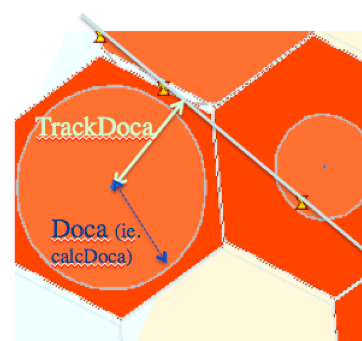
\includegraphics[width=0.2\textwidth]{pics/dcPattern10.png}
\caption{Illustration of DOCA computed from the corrected time and of the distance from the wire to the track
  (TrackDOCA).}
\label{fig:docas}
\end{figure}

In hit-based tracking, uncorrelated hit noise in the DCs is identified by a Simple Noise Removal (SNR) algorithm
and rejected. The SNR stores all of the data for a DC layer (112 sense wires for 36 layers in each of the six Forward
Detector sectors) bit-wise in an extended 128-bit word, with ``set'' bits corresponding to hits. The algorithm is
configured through parameters specifying the maximum tilt of a track segment and the number of missing layers
allowed in the formation of a segment. Using bit-wise operations on the extended words, the algorithm essentially
operates as a parallel processor on all 112 sense wires in a layer. This parallelism precludes the need of a wire
for-loop, which enables the algorithm to run in a negligible fraction of the total time for reconstruction. More to the
point, the SNR actually saves time by reducing the combinations that must be explored in the pattern-recognition
phase of the ensuing track-finding. An illustration of the SNR hit categorization in the DC is shown in
Fig.~\ref{fig:snr}.

\begin{figure}
\centering
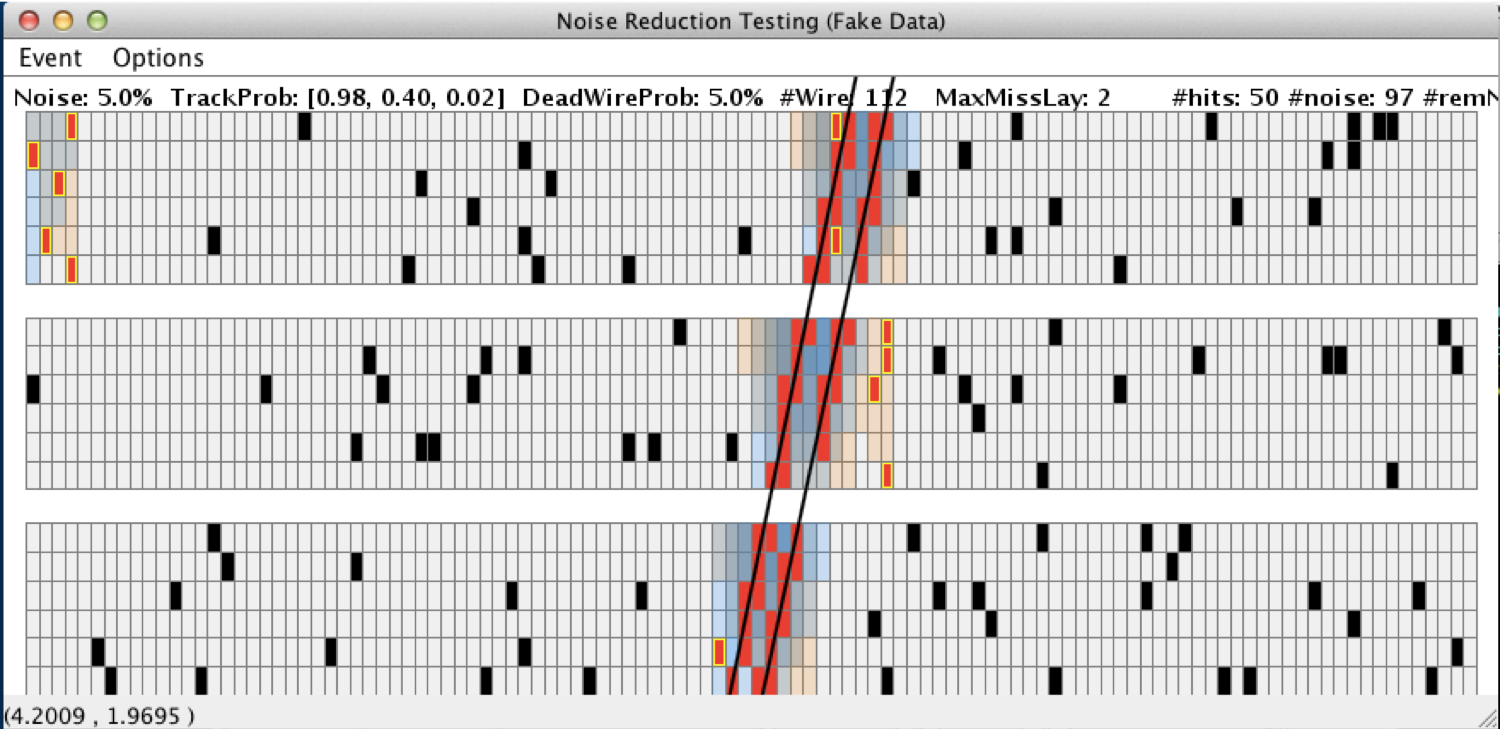
\includegraphics[width=0.48\textwidth]{pics/dcPattern9.png}
\caption{Illustration of DC hits categorized by the SNR algorithm. The black hits are identified as noise and
  discarded and the red hits are saved for further evaluation by the subsequent hit selection algorithms. The red
  hits with the yellow frames are saved noise (false alarms) and the shaded areas correspond to possible clusters.
  The darker shades correspond to a higher quality factor, hence a higher probability for hits on a track.}
\label{fig:snr}
\end{figure}

\subsubsection{Hit Clustering}

Within each of the six sectors of the CLAS12 Forward Detector, there are three sets of DCs that are referred to
as Region~1 (R1) upstream of the torus, Region~2 (R2) within the torus coils, and Region~3 (R3) downstream
of the torus (see Fig.~\ref{fig:dcTracks}). Each of the three detectors in each sector, R1, R2, and R3, consists of
two so-called ``superlayers'', which each contain six layers of 112 drift cells (or 6 wire layers). The hits remaining
after the SNR algorithm are grouped into clusters. Clusters are made up of adjacent hits within the wire layers of
a given DC superlayer. There can be at most two neighboring hits within a single wire layer, forming a
``double-hit''.\footnote{An additional hit in a layer is mostly out of time and has a drift time that when converted to a drift
  distance exceeds the cell size.}  However, up to two wire layers can be missing within a superlayer when attempting
to form a cluster.  This is to reduce tracking inefficiencies resulting from possible wire malfunctions or intrinsic
inefficiencies. It was found that requiring 4 out of 6 wire layers to form a cluster is sufficient to determine the
cluster shape, which is subsequently used to determine the track trajectory.

\begin{figure}
\centering
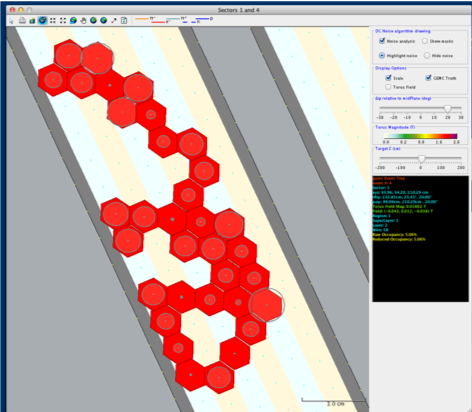
\includegraphics[width=0.4\textwidth]{pics/elooper.png}
\caption{Illustration of typical noise patterns in a single six wire layer superlayer in the DC displayed as seen using
  the CLAS12 Event Display {\it ced}. The hits shown are from a Monte Carlo electron event.}
\label{fig:eloop}
\end{figure}

Additional ``noise rejection'' algorithms are applied to the clusters to remove spurious hits that do not come from
a real track. So-called ``curler'' patterns as shown in Fig~\ref{fig:eloop} are typical for low-energy electrons in
the DC.  Therefore, a pruning algorithm was designed to remove them at an early stage of the reconstruction. The
algorithm is a counting method of the number of contiguous hits within a single wire layer of a superlayer.  In
Figs.~\ref{fig:eloop} and ~\ref{fig:strings} we also see another typical noise pattern that looks like horizontal
``strings'' of hits along a wire layer. An algorithm was developed following  the observation that high-momentum
tracks from hadrons typically cross the superlayers at a large angle, while ``curlers'' from low-momentum
background follow curling trajectories, with a significant part of the pattern lying within a single wire layer.
Subsequent algorithms  are employed for resolving overlapping segments.   

Overlapping segments are produced when the trajectories of two tracks cross each other or when the tracks are
almost parallel and very close to each other in a given region. A Hough Transform is employed to find hits on a line
in the cluster, which allows the cluster to be split into segments.  The resulting trimmed clusters are then fit to a
straight-line hypothesis, and those hits with acceptable residuals are kept and identified collectively as a
``track segment''. An illustration of the Hough Transform cluster selection algorithm is shown in Fig.~\ref{fig:hough}.

\begin{figure}[t]
\centering
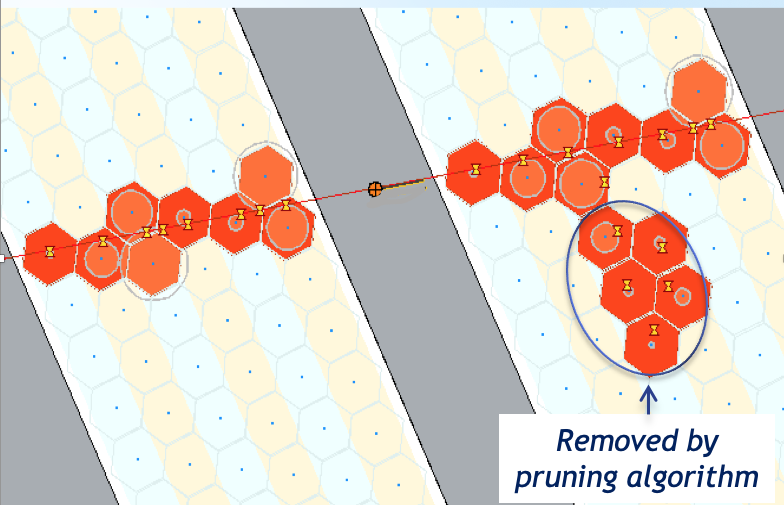
\includegraphics[width=0.4\textwidth]{pics/dcPattern2.png}
\caption{Illustration of hits rejected by the pattern recognition pruning algorithm in a Monte Carlo electron
  event. The circles superimposed on top of the DC cells indicate the DOCAs computed from the fully corrected
  times. The yellow hourglass symbols show the simulated track positions along the trajectory. The algorithm looks
  for ``strings'' of hits, such as shown in the third column of hits in the right-most superlayer in the figure. In this
  instance, the middle hit in this string would be rejected, leaving a set of four attached hits at the bottom part of
  the string that would subsequently be rejected since they would no longer be attached to the main cluster.}
\label{fig:strings}
\end{figure}

Subsequent hit pruning algorithms are employed at the time-based level. Figure~\ref{fig:dcsegs} illustrates the
selected hits belonging to a cluster (orange) and the hits rejected by the noise-finding algorithms.

\subsubsection{Pattern Recognition}

Fits to the segments with a linear function are a preliminary step to estimating a track trajectory. The track
parameters are estimated in the local coordinate system of DC from this trajectory.

Using the wire direction in a given superlayer along with the line fit to a segment in that superlayer, a plane can
be constructed. Thus pairs of segments in neighboring superlayers within one chamber (with superlayers of
$\pm$6$^\circ$ stereo angle) represent the intersection of two planes, which is a line whose coordinates are
evaluated midway between the two superlayers, and is a 6-dimensional object ($x$, $y$, $z$, and 3 angles) that
we call a ``cross''. A segment slope coincidence algorithm is used to match neighboring segments in a region (see
Fig.~\ref{fig:dcsegs}).  Selection cuts are subsequently applied on the reconstructed cross to ensure that it is
within the detector fiducial volume within resolution.

An additional pattern reconstruction algorithm matches segments within the even and odd numbered superlayers
in a given sector, respectively, to form a track candidate where an entire superlayer can be missing. The matching
algorithm returns an estimate of where the missing superlayer's hits should be and forms a ``pseudo-segment'' from
the wire locations corresponding to these hits. Subsequently a ``pseudo-cross'' is formed using the pseudo-segment
and the neighboring reconstructed segment in that region.

\begin{figure}
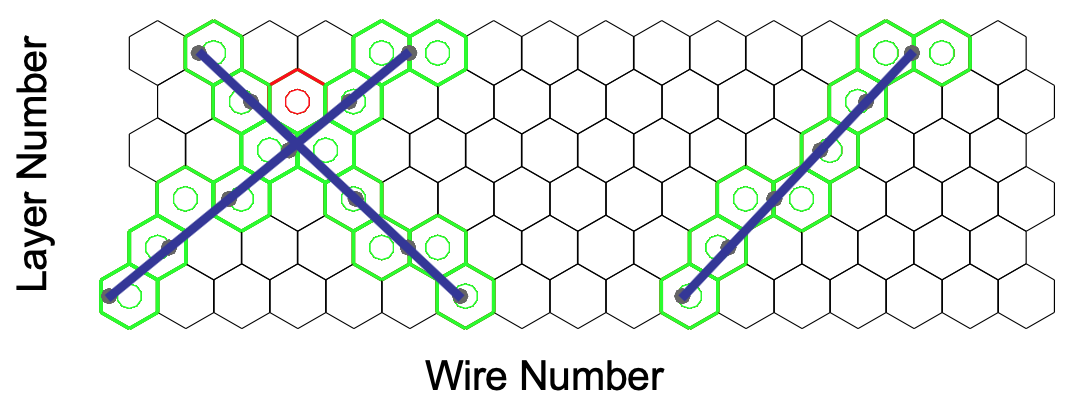
\includegraphics[width=0.45\textwidth]{pics/dcPattern14.png}
\caption{Illustration of selected clusters (left-most selected hits with superimposed lines) using a Hough Transform.
  Two track segments cross each other. The hits are separated into cluster candidates and fit using a local coordinate
  system as a function of layer and wire number. The selection is done without employing timing information.}
\label{fig:hough}
\end{figure}

The first stage of pattern-recognition consists of finding a track candidate from a set of 3 crosses (one each in R1,
R2, and R3) that are fit to a parabolic functional form to give a ``track candidate''. Using the parameters of the
parabolic function between the first and the third cross and obtaining the magnetic field intensity at each step along
this trajectory we obtain an estimate for $\int B dl$. From the local angles of the crosses in the $x-z$ plane for R1
($\theta_1$) and R3 ($\theta_3$), we estimate the track momentum ($p$) and the particle charge ($q$) as:

\begin{equation}
  \frac{q}{p} = \frac{\theta_3 - \theta_1}{v\int{B dl}},
\end{equation}

\noindent
where the angles are in radians, the magnetic field intensity ($B$) is in Tesla, and the path length ($dl$) is in cm.
The conversion factor $v$ corresponds to the speed of light. The cross position and angles in DC R1, together with
the momentum and the charge, provide all of the necessary information to define the track parameters at a given
location in the detector, and therefore to start the track fitting.

\begin{figure}[t]
\centering
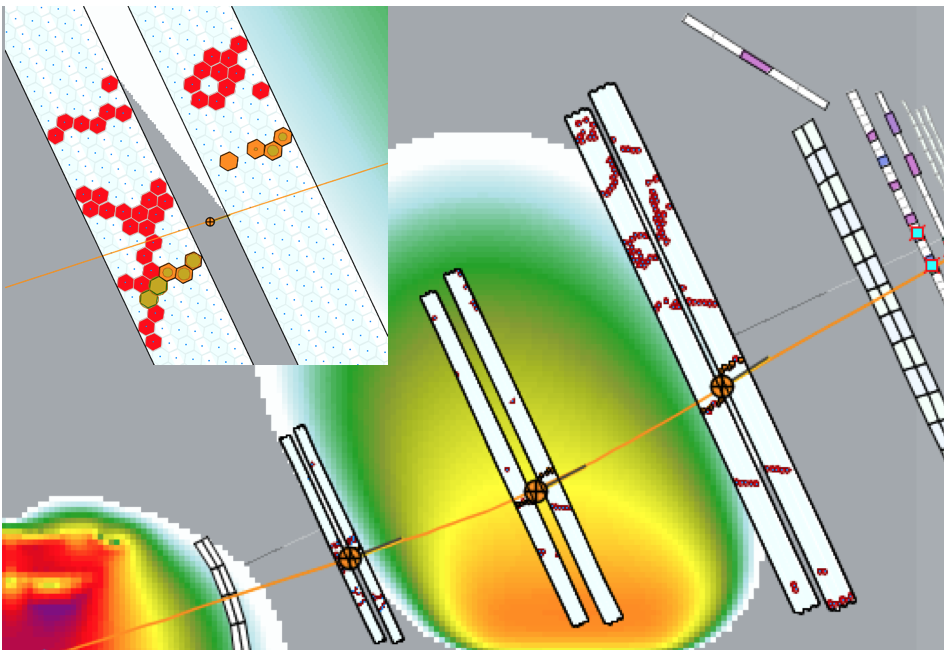
\includegraphics[width=0.4\textwidth]{pics/dcPattern13.png}
\caption{Illustration of rejected hits (red hexagons) and accepted hits (orange hexagons) by the forward tracking
  pattern recognition algorithm using Monte Carlo data. The red cells correspond to hits not rejected by the SNR
  algorithm and the circles represent the calculated DOCAs.  The superimposed lines show the local fits to the
  DOCAs. The filled circle between the superlayers of a given region (R1, R2, or R3) represents the 3-D point
  (called a ``cross'') obtained from the local fits to the DOCAs taking into account the direction along the wires. The
  offset between the segments composing the cross comes from the projection at the $y=0$ plane. The cluster shown
  on the right-most superlayer is an example of a ``looper'' and shows how this category of cluster has the potential
  to bias the track. The second cluster used to form the cross yields an incorrect slope resulting from a wrong hit
  used in the fit.  Subsequently, the ``looper'' search algorithm rejects the entire cluster and only the first cluster
  is used to fit the track. The fitted track trajectory is represented by the orange line. The upper figure is a zoomed
  view into the track trajectory in R1.}
\label{fig:dcsegs}
\end{figure}

\subsubsection{Track Fitting}
\label{sec-trackfitting}

The output of the pattern recognition is a seed with initial parameters used to start the track propagation from one
measurement site to the next in the fit. The track fitting uses a Kalman Filter method with a 5-parameter track
representation ($x$, $y$, $tx$, $ty$, $q$/$p$) called the track state vector, defined in a local coordinate system
with the $z$-axis perpendicular to the DC wire planes. Here $q$ is the track charge, $tx=p_x/p_z$, $ty=p_y/p_z$,
and $p_x$, $p_y$, and $p_z$ represent the $(x,y,z)$ components of the track momentum in the local analysis frame.
In the analysis frame the state vector and the measurement are defined at each layer for which there is a hit on a
track. Hence, as in Ref.~\cite{spiri}, we can express the equations of motion of the track in the torus field and the
propagation of the state vector covariance matrix as derivatives with respect to $z$. In the DC, the magnetic field
components are mostly along the $y$ coordinate (along the wires) in the analysis frame. The trajectory of the particle
in the analysis frame is given by:

\begin{eqnarray}
dx/dz  &=& tx, \nonumber \\
dy/dz  &=&  ty, \nonumber \\
dtx/dz &=& q \cdot v \cdot \sqrt{1 + {t_x}^2 + {t_y}^2}  \nonumber \\
       &\cdot&\!\!\!\!\! [t_y\cdot (t_x B_x + B_z) - (1 + {t_x}^2 ) B_y],  \nonumber \\
dty/dz  &=&  q \cdot v \cdot \sqrt{1 + {t_x}^2 + {t_y}^2} \nonumber \\
      &\cdot&\!\!\!\!\! [-t_x\cdot (t_y B_y + B_z) + (1 + {t_y}^2 ) B_y], \nonumber \\
q  &=&  q_0,
\end{eqnarray}

\noindent
where the initial values at the starting point $z = z_0$ are $x = x_0$, $y = y_0$, $t_x = t_{x0}$, $t_y = t_{y0}$,
and $q = q_0$.

The above equations are solved numerically using a fourth-order Runge-Kutta integration method in order to
propagate the state vector from the DC plane at $z_0$ to the next one at $z$.  The state vector covariance
matrix is propagated along with it by computing the Jacobian matrices as in Ref.~\cite{spiri}, again solving using
a fourth-order Runge-Kutta method. The Jacobian matrix terms contribute to the propagator matrix used to
compute the Kalman gain. The propagated covariance matrix takes into account multiple scattering through the
known material layers of the DC tracking volume.

The non-zero components of the multiple scattering matrix are:

\begin{eqnarray}
Cov (t_x , t_x) &=& (1+{t_x}^2 )\cdot (1+{t_x}^2 + {t_y}^2 )\cdot {\theta_0}^2 , \nonumber \\
Cov (t_y , t_y) &=& (1+{t_y}^2 )\cdot (1+{t_x}^2 + {t_y}^2 )\cdot {\theta_0}^2 , \nonumber \\
Cov (t_x , t_y) &=&  t_x t_y\cdot (1+{t_x}^2 + {t_y}^2 )\cdot {\theta_0}^2 ,
\end{eqnarray}

\noindent
where,

\begin{eqnarray}
  {\theta_0} &=& \frac{13.6}{\beta pc}\sqrt{\frac{t}{X_0}\sqrt{1+{t_x}^2+{t_y}^2}}\\
  &\times&\left[ {1+0.038~\ln \left({\frac{t}{X_0}\sqrt{1+{t_x}^2+{t_y}^2}}\right) }\right] \nonumber
\end{eqnarray}

\noindent
as given by the Highland-Lynch-Dahl formula~\cite{Highland-Lynch-Dahl}. The radiation length $X_0$ is computed
as an effective radiation length corresponding to the gas mixture in the DC wire layer. Air is assumed outside of
the DC volumes. The term $t$ represents the path length traversed by the track.

At each plane the state vector is mapped onto a measurement, which corresponds to the drift distance to the
wire in a given DC plane.  In instances where there are two hits associated with the track in a given wire layer
(i.e. the track goes in between the wires), the information from both hits is included in the fit. The measurements
used in the fit take into account the left/right position of the track with respect to the wire.

Time corrections are applied after hit-based tracking to account for the event start time, cable delays,
propagation times along the wires, event flight times to the hit location along the wires, $\beta$-dependent
corrections, and the effect of the magnetic field on the cell isochrones that modify the drift times~\cite{dc-nim}.

After the times are corrected, the drift distance is computed using tabulated distance-to-time multi-dimensional
arrays. The drift distances are computed using a multi-dimensional interpolation method using the segment local
angle (i.e. the entrance angle of the track in the cell), the value of the magnetic field at the location of the hit, and
the corrected times. The Kalman fit is redone at the time-based level using the hits with corrected times and the
computed drift distances. A graphical representation of tracks in {\it ced} is shown in Fig.~\ref{fig:dcTracks}. This
is a typical event for the nominal running conditions of CLAS12. 

\subsection{Central Tracking}
\label{sec:cvt}

Tracks whose polar angle is between $40^\circ$ and $135^\circ$ are reconstructed by the Central Vertex Tracker
(CVT). The CVT consists of twelve cylindrical layers of tracking detectors, numbered from 1 for the innermost layer
to 12 for the outermost layer. The subset of tracking detectors forming layers 1 to 6 are silicon strip sensors within
the CLAS12 Silicon Vertex Tracker (SVT)~\cite{svt-nim}. Layers 7 to 12 are made of Micromegas tiles within the
Barrel Micromegas Tracker (BMT)~\cite{mm-nim}. The entire CVT surrounds the target and sits in the 5~T solenoid
field. The SVT is made from 3 concentric rings of double-layer silicon sensors with a graded strip stereo angle from
0$^\circ$ to 3$^\circ$ (with 0$^\circ$ along the beamline $z$-axis) and a readout pitch of 156~$\mu$m. The BMT
consists of 3 cylindrical detectors with strips along the $z$-axis (called the BMT-Z layers) and 3 cylindrical layers
with circular layers with circular strips perpendicular to the $z$-axis (called the BMT-C layers). Each layer is divided
into three 120$^\circ$ sectors.

The revolution axis of the CVT coincides with the ideal beam axis, which defines the $z$-axis of the CVT. The
$y$-axis points upward in the laboratory frame and the $x$-axis is defined to form a right-handed coordinate
system. The origin of the CVT coordinate system matches the center of the nominal CLAS12 target center. An
illustration of the CVT detector with {\it ced} is shown in Fig.~\ref{fig:cvt}.

\begin{figure}
\centering
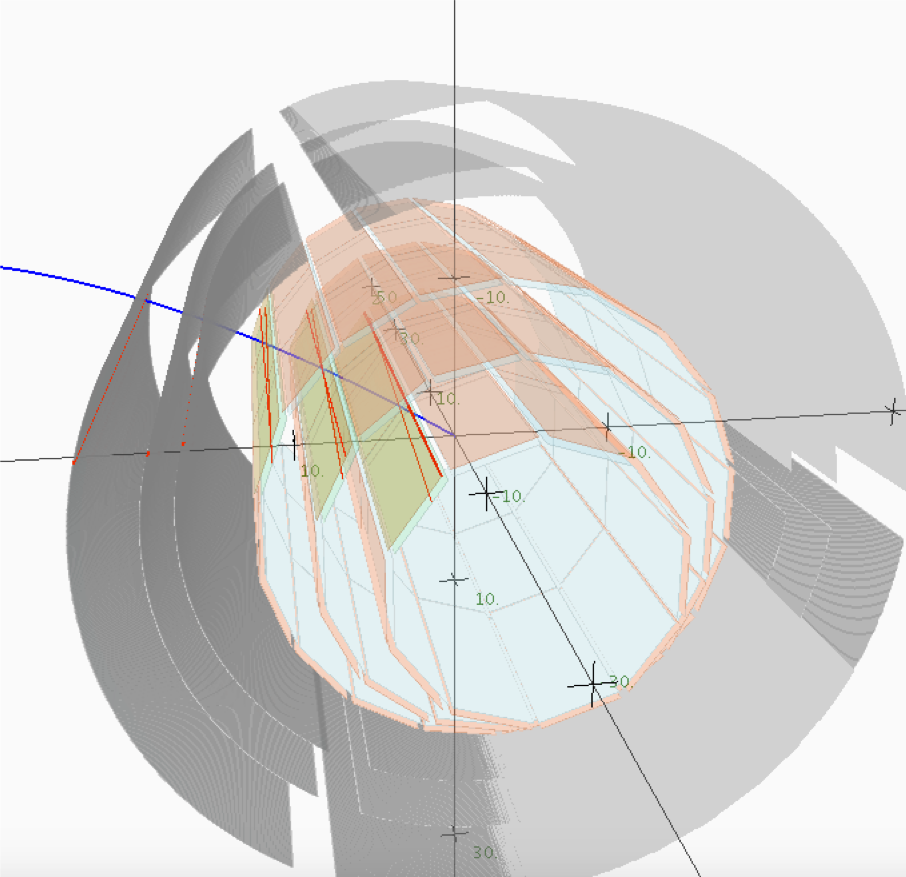
\includegraphics[width=0.5\textwidth]{pics/cvt.png}
\caption{Event display view of the CVT detector showing the 3 inner double layers of the SVT (in red) and the
  BMT layers (in gray). The red lines in the upper left of the SVT in this view represent active SVT strips
  corresponding to hits on a track.}
\label{fig:cvt}
\end{figure}

\subsubsection{Hit Clustering}

The first step of the tracking algorithm is the formation of clusters from the raw hits. The SVT raw 3-bit ADC
values are transformed into deposited charge by randomly sampling a Landau distribution determined from
test-bench data. A cluster is a collection of contiguous hit strips. Its centroid is either given by spatial information
(a $z$-coordinate for the BMT-C detectors in which strips are arcs at constant $z$ or $xy$-coordinates for the
BMT-Z detectors in which strips are parallel to the $z$ axis) or an average strip number for the SVT. This centroid
is derived by performing an average of the relevant strip information, weighted by the maximum of the ADC pulse for
the Micromegas strips or the equivalent deposited charge for the SVT. The time information associated with each hit
is currently not used.

Before feeding all of the CVT clusters to a pattern recognition algorithm, spatial coordinates must be associated with
the SVT clusters. As described in Ref.~\cite{svt-nim}, the SVT layers are mechanically paired and consequently form
three regions. The readout strips of the inner and outer layer of each region make a $3^\circ$-stereo angle. By
associating one cluster of the inner layer with one cluster of the outer layer, and by assuming that an infinite
momentum track perpendicularly crossed the two layers, a preliminary assignment for the $(x,y,z)$ coordinates of
the particle between the two layers is derived for this cluster pair. This pairing is performed over all clusters of the
inner layer with all clusters of the outer layer. Pairs whose $(x,y,z)$ coordinates are outside of the physical SVT
sensor space are automatically removed from the list of $(x,y,z)$ candidates. If one of the two layers of a region has
no hit that can be associated with a particle, then the information of the active layer is simply ignored for the
remainder of the reconstruction process.

\subsubsection{Pattern Recognition}

The trajectory of a charged particle in a solenoidal magnetic field is an helix. Because the BMT detectors offer
either $xy$- or $z$-coordinates but never both, the pattern recognition cannot be performed in 3 dimensions. For
particles of large enough momentum (perpendicular momentum $p_\perp \> 0.25$~GeV for a 5~T solenoidal magnetic
field), the $xy$-projection of a helix is a circle, and the $rz$-projection is a straight line (where
$r = \sqrt{x^2 + y^2}$). Therefore, a first pattern recognition algorithm is run in the $xy$-plane to look for circles
and then a second pattern recognition algorithm is run in the $rz$-plane to search for straight lines.

The two pattern recognition algorithms are a modified version of the cellular automaton (CA) algorithm developed
by the HERA-B Collaboration~\cite{CA-HeraB}. Here, the elementary cell of the CA is defined as a segment that
connects two 2-D points. In the $(x,y)$ plane, cells are formed with SVT and BMT-Z $xy$-information. Two
$xy$-clusters form a cell if the angular distance between them is lower than a defined threshold. This threshold
has been derived by maximizing the reconstruction efficiency on a single track Monte Carlo simulation with
background extracted from the data. Two clusters cannot form a cell if they are separated by more than one layer.
Finally, the CA is run sector-by-sector in the BMT and, as a consequence, a cell cannot be formed with two clusters
residing in different BMT sectors.

The subsequent step is the ``neighbor'' finding. Cell ``a'' is a neighbor of cell ``b'' if they share one cluster and
if the layer numbers in ``b'' are higher than those in ``a''. Tuned on single-track Monte Carlo simulation data
without background, cuts on the dot product between the cell directions are applied as neighbor-forming criteria.
Once the neighborhood of a cell is defined, the CA is evolved over an $N$-evolution stage. For evolution stage $n$,
the state of all cells is updated according to $S_n = max(S_{n-1}^j) + 1$, where $S_{n-1}^j$ is the state of the
$j^{th}$-neighbor of the considered cell at evolution time $n-1$. Therefore, at evolution stage $N$, the cells with
the highest state are further outward than the cells with a smaller state. \color{red} \textbf{Caption of a figure
  to be produced to explain CA evolution} \color{black}

Track candidates in the $(x,y)$ plane are then formed starting from the highest state cells and following the
neighbor chain with $\Delta S = 1$. In case of multiple neighboring cells with the same state, the one that has
the smaller dot product with the original cell is chosen.

Due to the poor $z$-resolution of the preliminary SVT 3-D points, the search for candidates in the $(r,z)$ plane is
performed by only using the $z$-clusters of the BMT. The CA algorithm trivially returns the track segments of two
or three BMT-C clusters. Due to the orthogonality of the BMT-C and BMT-Z readout, all of the $(r,z)$ segments of
a BMT sector are combined with the $(x,y)$ candidates in the same sector. A line is fitted on the BMT-C hits and
its intersections with the three SVT regions are computed. If the distance between the expected intersection and
the preliminary 3-D point in the SVT region is greater than two millimeters, then the two SVT clusters forming this
preliminary point are removed from the track candidate.

\subsubsection{Track Fitting}

Each track candidate is then passed to a Kalman filter. The state vector to describe a helix is formed by five
parameters $(\varphi_0, d_0, \kappa, z_0, \tan(\theta_{dip}))$, where:

\begin{itemize}
\item $d_0$ is the $(x,y)$ distance of closest approach to the CVT revolution axis;
\item $\varphi_0 = {\rm atan}(p_y/p_x)$ at closest approach angle to the CVT revolution axis;
\item $\kappa=q/p_\perp$ and $q$ is the electric charge of the particle and $p_\perp=\sqrt{p_x^2+p_y^2}$ is
  the transverse momentum;
\item $z_0$ is the distance along the $z$ axis to the CVT center;
\item $\theta_{dip}$ is the polar angle between the track and the $xy$-plane.
\end{itemize}

To initialize the Kalman Filter, a first estimate of these parameters is obtained from:

\begin{itemize}
\item a circle fit in the $xy$-plane with preliminary SVT 3-D points and BMT $xy$-clusters for $d_0$,
  $\varphi_0$, and $\kappa$. To improve the initialization of the fit, the point (0,0) (on the ideal beam $z$-axis)
  is included in the fit with an accuracy of 100~$\mu$m.
\item a line fit in the $rz$-plane using only the $z$-clusters of the Micromegas to initialize $z_0$ and $\theta_{dip}$.
\end{itemize}

The covariance matrices of the two fits are merged into a 5$\times$5 matrix to initialize the covariance matrix
for the Kalman filter. Following the transport equations in Ref.~\cite{ILC-Tracking}, the state vector is
propagated from the CVT revolution axis to the outermost layer of the CVT, filtering at each measurement
composing the track candidate. Once the last measurement is reached, the state vector and covariance matrix
are brought back to the CVT revolution axis as they are and the transport/filtering process is re-run. A maximum
of five iterations is performed to make sure of the convergence of the filtering process.

\subsection{Tracking Performance}

The momentum resolutions in the central and forward trackers as a function of momentum are shown in
Figs.~\ref{fig:respcvt} and~\ref{fig:respdc}, respectively. The distributions are fit with a function of the form
$\sqrt{a+b x^2+c/(1+d/x^2)}$.  The resolutions achieved are well within the design specifications and the
difference in magnitude between the central and the forward trackers is due to the intrinsic resolutions of these
detectors. 

\begin{figure}
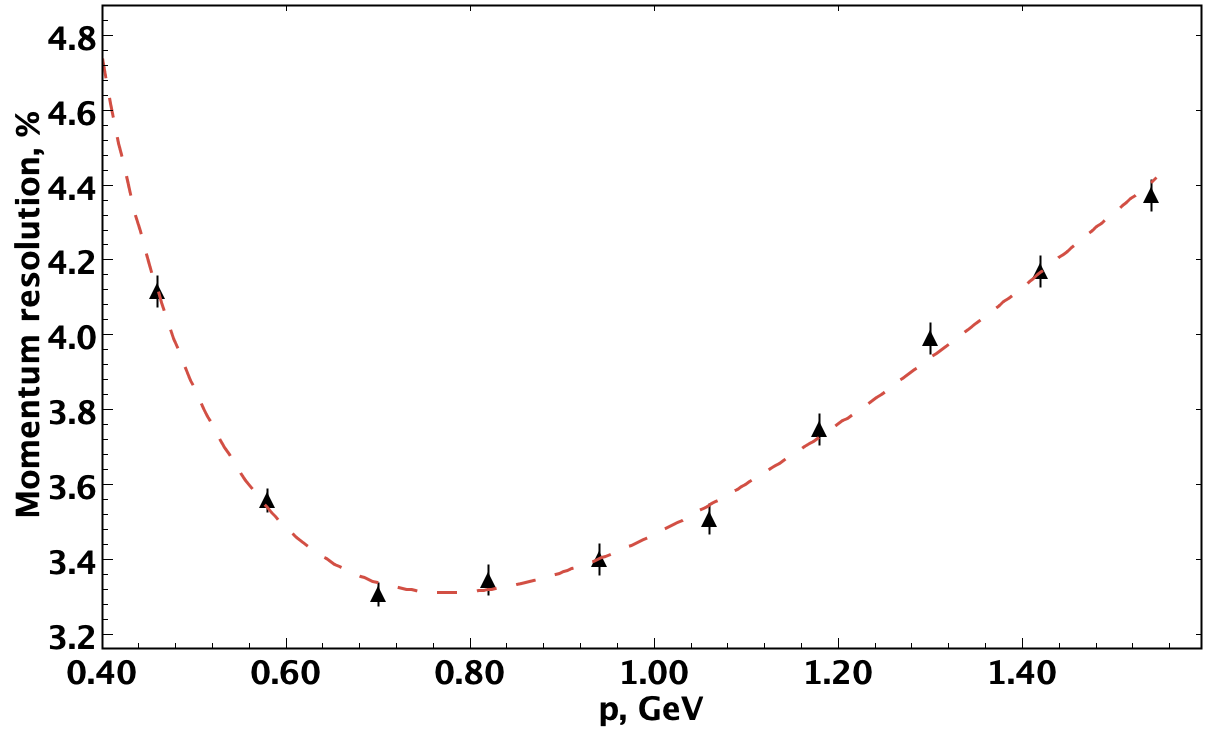
\includegraphics[width=0.45\textwidth]{pics/fddegipekmpjjiho.png}
\caption{Momentum resolution vs. momentum of simulated protons in the CVT without background.}
\label{fig:respcvt}
\end{figure}

\begin{figure}
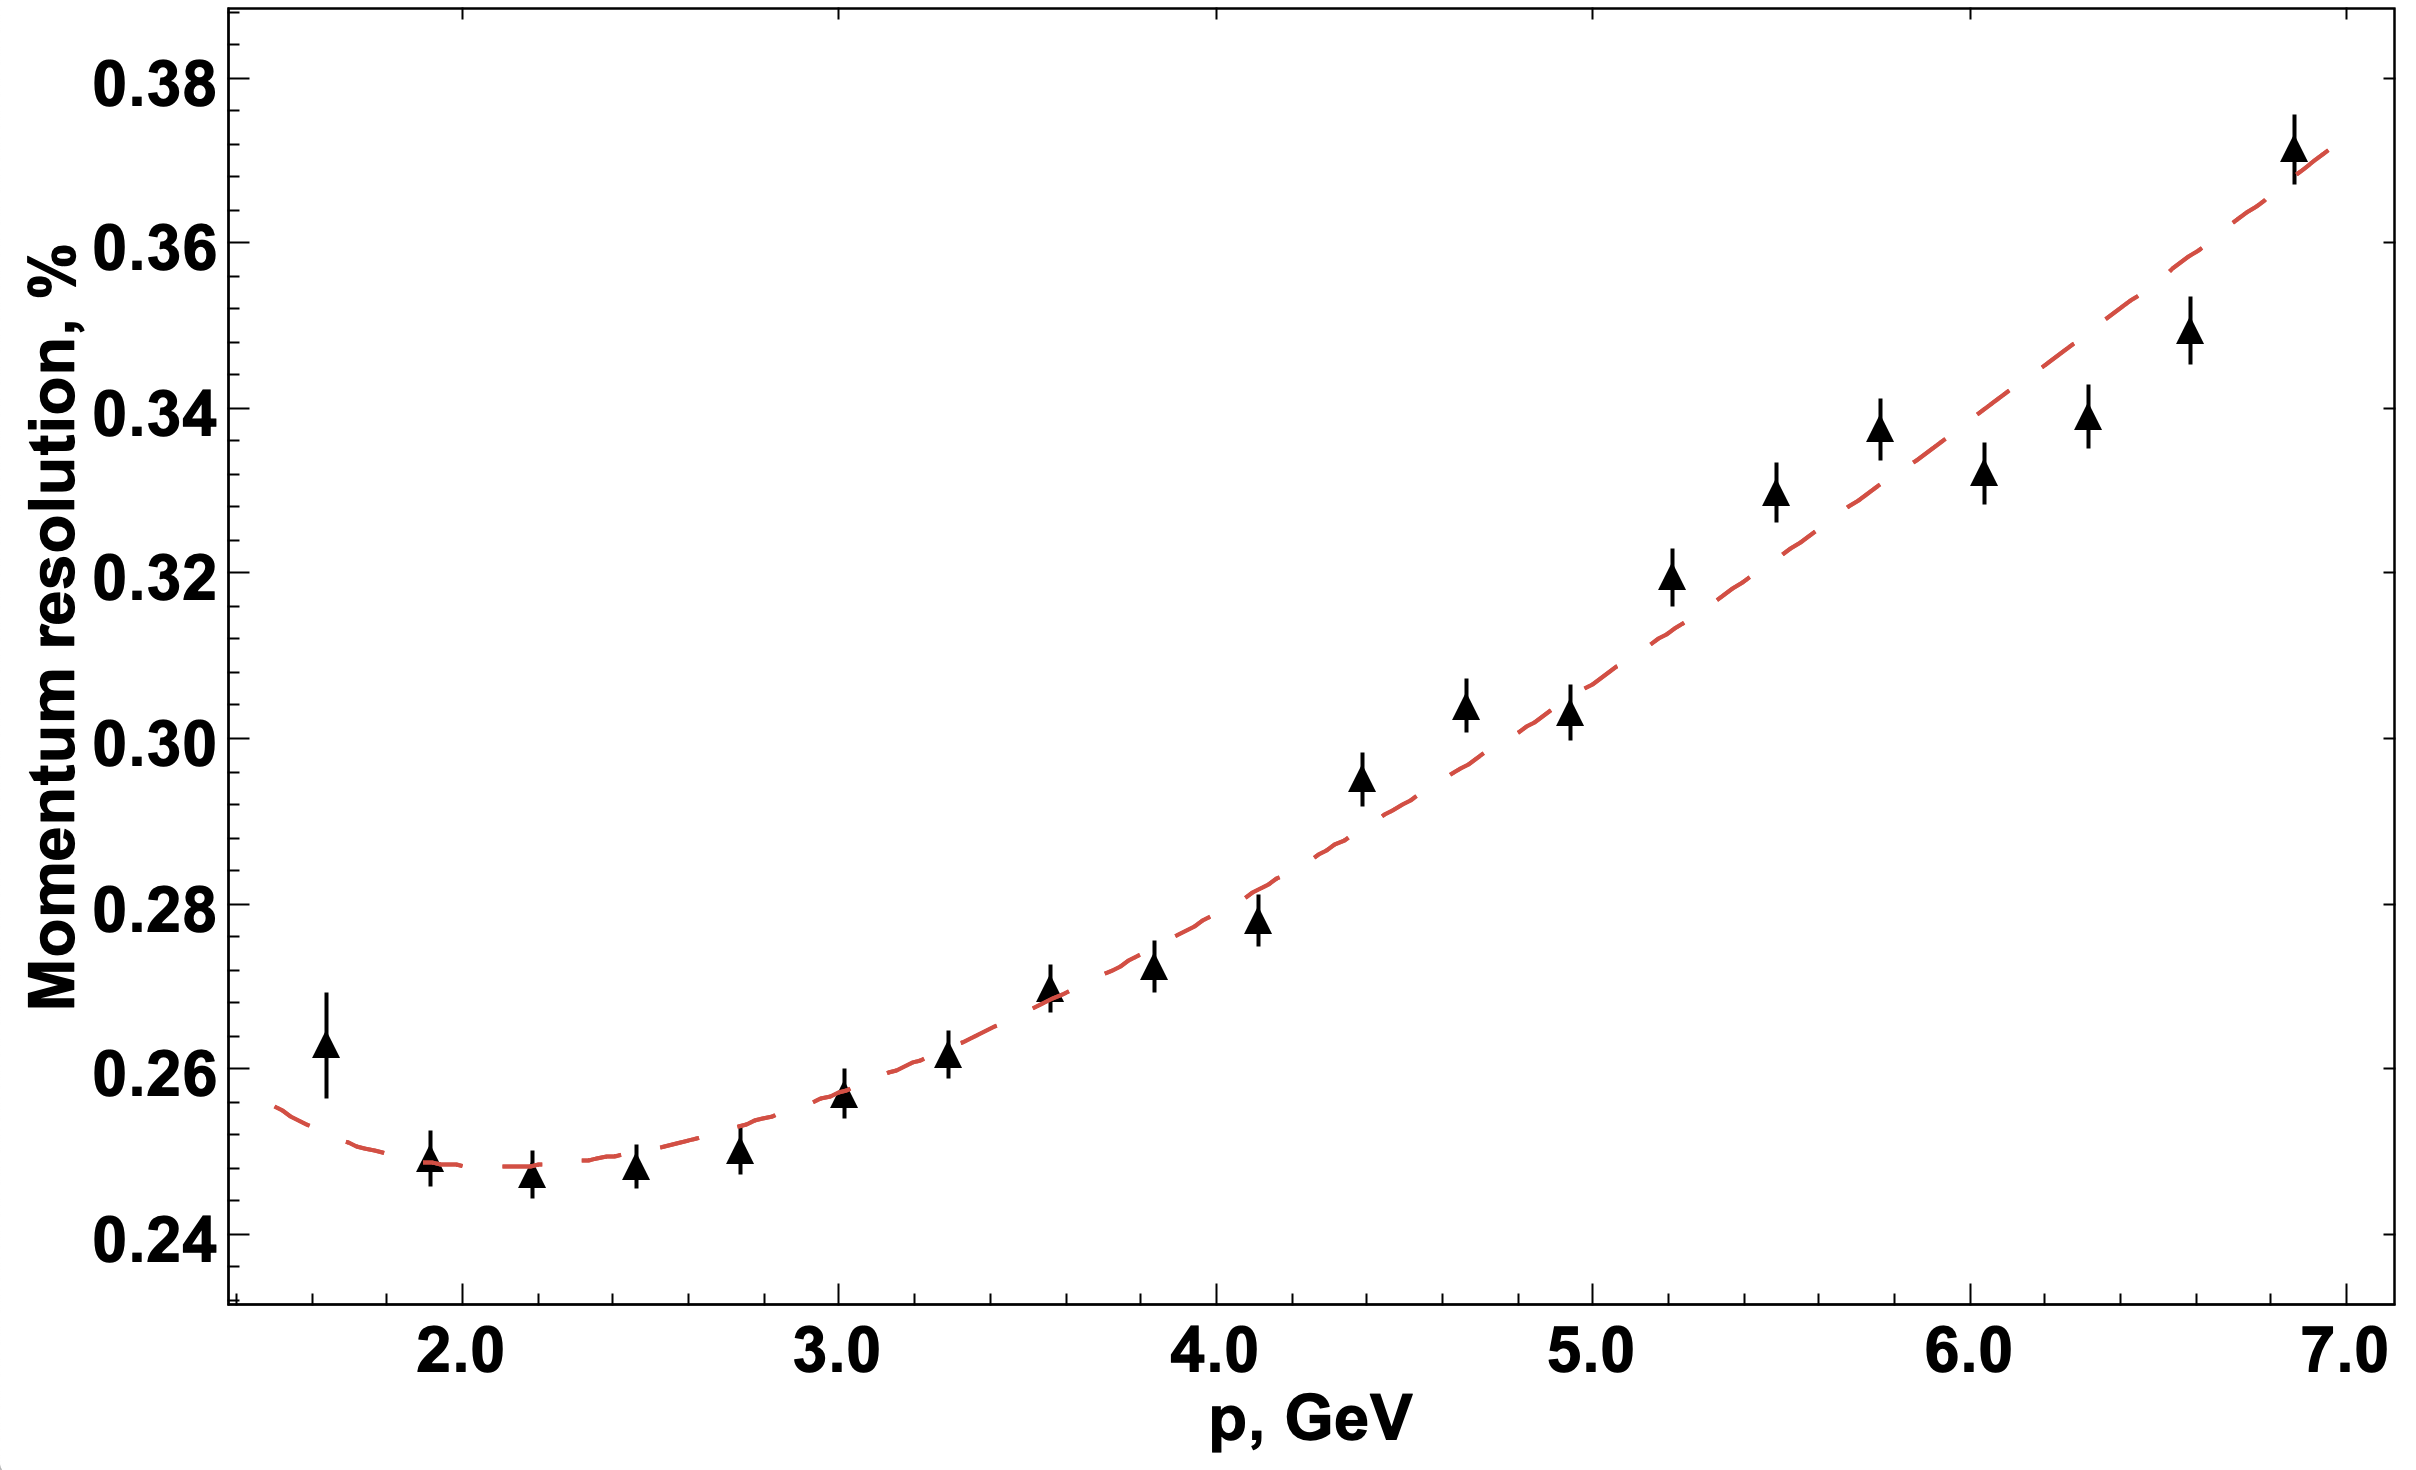
\includegraphics[width=0.45\textwidth]{pics/DCRes.png}
\caption{Momentum resolution vs. momentum in the DC evaluated using pions simulated at
  $\theta =15^\circ \pm 5^\circ$ and at $\phi = 0 \pm 5^\circ$ without background.}
\label{fig:respdc}
\end{figure}

For the central tracking, an average CVT tracking efficiency of 91\% is obtained from a simulated proton sample with
momentum range from 0.4 to 1.6~GeV. A drop of efficiency is observed for tracks with momenta less than 600~MeV
as these low momentum tracks tend to not leave enough hits in the detector for the pattern recognition algorithm to
identify a track.  

For the forward tracking, the momentum resolution in the DC is evaluated using tracks simulated at
$\theta =15^\circ \pm 5^\circ$ and at $\phi = 0 \pm 5^\circ$ (sample~1), to ensure that most tracks are within the
sensitive volume. Furthermore, the DC momentum resolution is correlated with the polar angle since the track
curvature is determined from the magnetic field intensity, which is higher at lower angles in the torus field, as can
be seen from Fig.~\ref{fig:restheta}, corresponding to tracks simulated at $p=4\pm 1$~GeV,
$10^\circ \leq \theta \leq 25^\circ$ and $\phi = 0 \pm 5^\circ$ (sample~2).

\begin{figure}
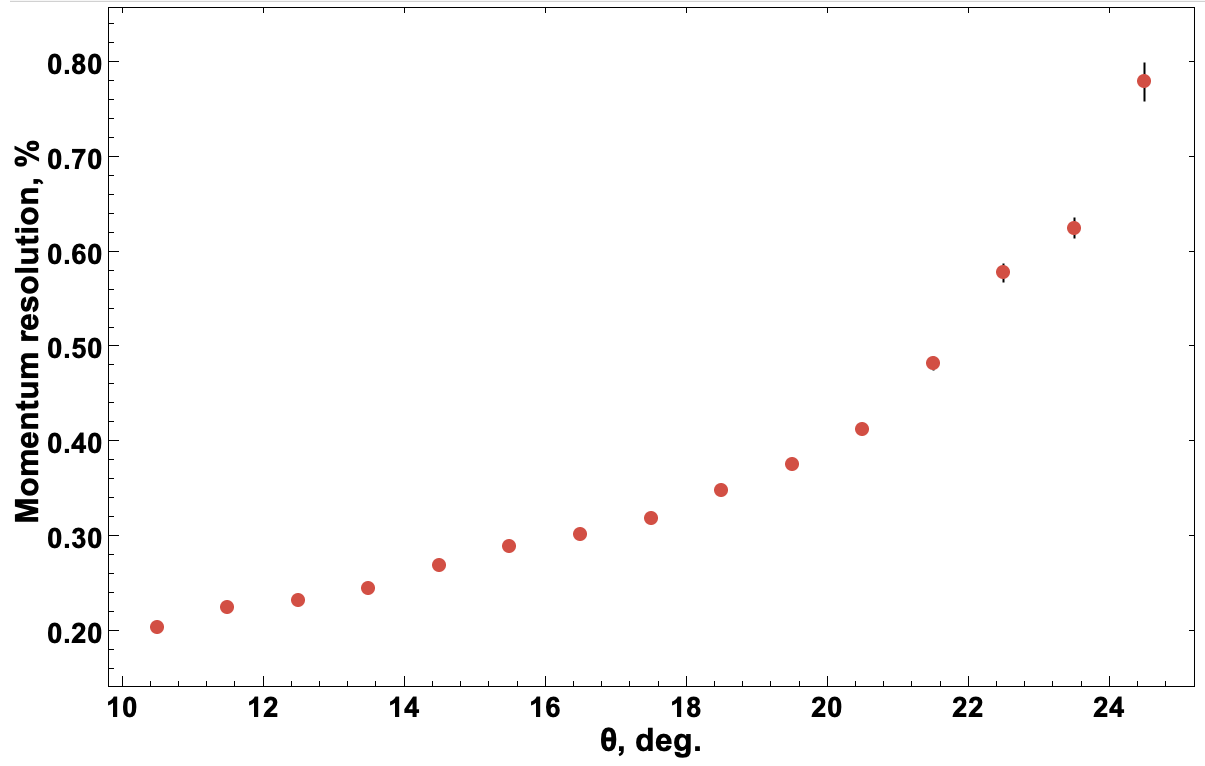
\includegraphics[width=0.45\textwidth]{pics/DCRes2.png}
\caption{Momentum resolution vs. polar angle in the DC evaluated using pions simulated at $p=4\pm 1$~GeV,
  $10^\circ <\leq \theta \leq 25^\circ$ and $\phi = 0 \pm 5^\circ$ without background.}
\label{fig:restheta}
\end{figure}

These resolutions are obtained from a Monte Carlo sample that does not include out of time backgrounds or
misalignments of the tracking volumes. A dedicated study that involves merging random background data with
low luminosity data is described in Ref.~\cite{clas12-nim}.

The tracking efficiency for inbending and outbending tracks in the torus field calculated from sample~1 is shown in
Fig.~\ref{fig:trkeff}. Inbending tracks suffer from a loss in tracking efficiency for momenta generated below
1.8~GeV at the time-based level due to lack of matching with the outer detectors. These tracks miss the sensitive
volumes of the Forward Time-of-Flight (FTOF) system, which is required to extract the time-correction information
needed for time-based tracking. The tracks do however pass the hit-based tracking requirement. The efficiency
loss due to the aforementioned effect can be seen by comparing the (light) blue to the (dark) red distribution. In
the momentum range from 1.8 to 7.5~GeV, the time-based tracking efficiency is 98\%, while in the range from
1.4 to 7.5~GeV, the hit-based tracking efficiency is 99\%. For outbending tracks (see Fig.~\ref{fig:trkeff}(bottom)),
both the hit-based and time-based tracking efficiencies are flat as a function of momentum and on the order of 99\%. 

\begin{figure}[t]
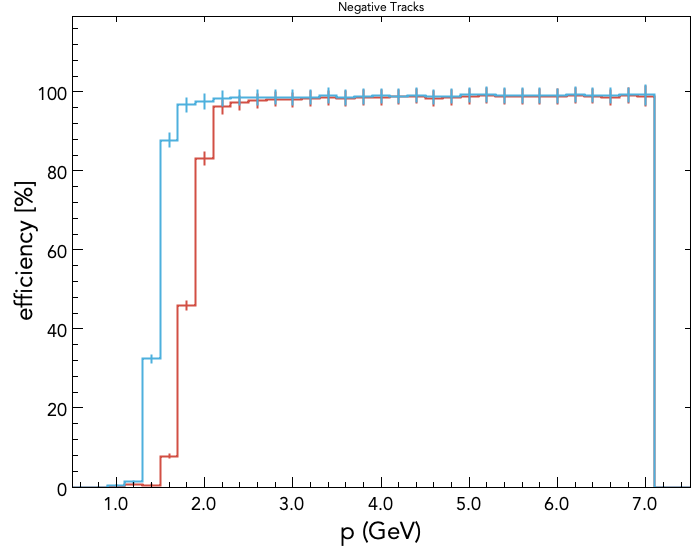
\includegraphics[width=0.45\textwidth]{pics/DCTrkgEffNegTrks.png}
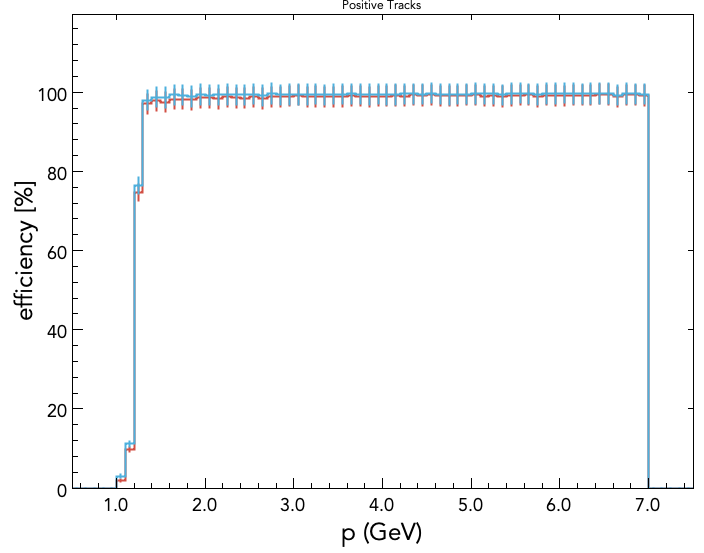
\includegraphics[width=0.45\textwidth]{pics/DCTrkgEffPosTrks.png}
\caption{DC tracking efficiency as a function of momentum evaluated using  (top) negative and (bottom) positive pions
  simulated at $\theta =15^\circ \pm 5^\circ$ and at $\phi = 0 \pm 5^\circ$. The (light) blue and (dark) red distributions
  correspond to the hit- and time-based tracking efficiencies, respectively.}
\label{fig:trkeff}
\end{figure}

The polar angular dependence of the DC tracking efficiency obtained from sample~2 is shown in
Fig.~\ref{fig:trkeffinoutb}. The (light) green histogram corresponds to outbending tracks. The efficiency is flat
in the angular range from 10$^\circ$ to 25$^\circ$ for outbending tracks, while there is a loss of tracks below
15$^\circ$ for the inbending tracks. As discussed above, this is due to tracks missing the outer detectors.  

\begin{figure}
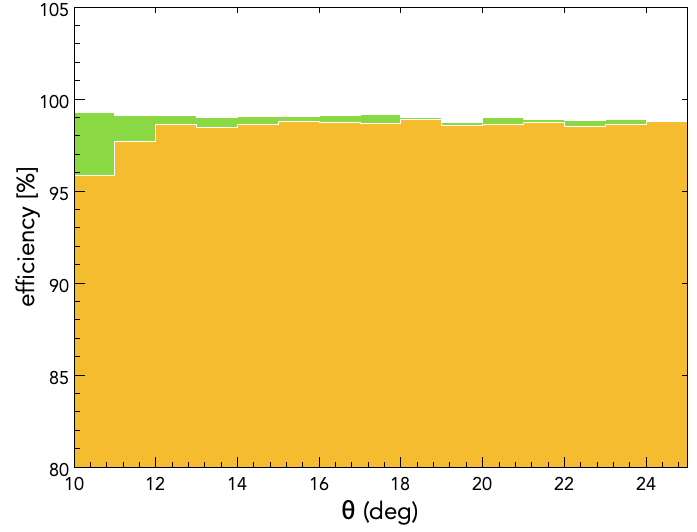
\includegraphics[width=0.45\textwidth]{pics/DCTrkEffvsThetaInandOutbenders.png}
\caption{DC tracking efficiency as a function of polar angle evaluated using  pions  simulated at $p=4\pm 1$~GeV,
  $10^\circ \leq \theta \leq 25^\circ$ and $\phi = 0 \pm 5^\circ$.}
\label{fig:trkeffinoutb}
\end{figure}
